\documentclass[10pt]{article}
\usepackage[utf8]{inputenc} 
\usepackage{enumerate}
\usepackage{amsmath}
\usepackage{graphicx}

\begin{document}
\begin{center}{
\huge\textbf{Laboratorio 1 \\ Computación Científica I}} \\
\bigskip
\textit{I) Representación Punto Flotante \\ II) Pérdida de significancia}

\vspace*{5.0 in}
\small{INTEGRANTES:} \\
\small{Oscar Rencoret oscar.rencoret@alumnos.usm.cl 2011735352-8} \\
\small{Ximena Rojas ximena.rojas@alumnos.usm.cl 201173568-4}
\end{center}

\newpage

\section{Introducción}
Este informe tiene como objetivo resolver y analizar los ejercicios propuestos que ponen en evidencia las limitaciones de realizar cálculos aritméticos en un computador y que se deben tener en cuenta al realizar operaciones aritméticas.

\section{Pequeña descripción de los experimentos}
\begin{itemize}
\item Se pone a prueba la precisión del ordenador, realizando operaciones aritméticas en ordenes de magnitud alrededor del $\epsilon_{match}$ 
\item Se representan gráficamente los números decimales en notación de punto flotante con la finalidad de evidenciar la pérdida de precisión.
\end{itemize}

\section{Parte I: Representación Punto Flotante}

\subsection{Pregunta 1}

\begin{enumerate}[a)]
\item Calcule las distancias aritméticamente.\\
Aritméticamente las sumas dan como resultado:
\begin{enumerate}[(i)]
\item 
\begin{equation}
\begin{aligned}
((1 + 2^{-52}) - 1) + 2^{-54} + 1 &= 2^{-52} + 2^{-54} + 1 \\
2^{-52} + 2^{-54} + 1 &= 2^{2} * 2^{-54} + 2^{-54} + 1 \\
2^{2} * 2^{-54} + 2^{-54} + 1 &= 2^{-54}( 2^{2} + 1) + 1 \\
2^{-54}( 2^{2} + 1) + 1 &= 2^{-54} * 5 + 1 \\
5 * 2^{-54} + 1 &= 1.000000000000000277555756
\end{aligned}
\end{equation}
\begin{equation}
\begin{aligned}
((1 + 2^{-54}) - 1) + 2^{-52} + 1 &= 2^{-54} + 2^{-52} + 1\\
2^{-54} + 2^{-52} + 1 &= 2^{-54} + 2^{2} * 2^{-54} + 1 \\
2^{-54} + 2^{2} * 2^{-54} + 1 &= 2^{-54}( 1 + 2^{2}) + 1\\
2^{-54}( 1 + 2^{2}) + 1 &= 2^{-54} * 5 + 1 \\
5 * 2^{-54} + 1 &= 1.000000000000000277555756
\end{aligned}
\end{equation}

\item 
\begin{equation}
\begin{aligned}
(5 - 4) + 2^{-52} &= 1 + 2^{-52} \\
1 + 2^{-52} &= 1.000000000000000222044605
\end{aligned}
\end{equation}
\begin{equation}
\begin{aligned}
5 - (4 - 2^{-52}) &= 5 - 4 - 2^{-52}\\
5 - 4 - 2^{-52} &= 1 - 2^{-52} \\
1 - 2^{-52} &= 0.999999999999999777955395
\end{aligned}
\end{equation}

\item 
\begin{equation}
\begin{aligned}
(2^{53} + (-2^{53})) + (1 + 0.5 + 0.25) &= (2^{53} - 2^{53}) + 1.75 \\
(2^{53} - 2^{53}) + 1.75 &= 1.75
\end{aligned}
\end{equation}
\begin{equation}
\begin{aligned}
(2^{53} + (1 + 0.5 + 0.25)) - 2^{53} &= 2^{53} + 1.75 -  2^{53} \\
2^{53} + 1.75 -  2^{53} &= 1.75
\end{aligned}
\end{equation}

\end{enumerate}

\item Con la ayuda de \textit{Python} o \textit{Matlab}, calcule nuevamente las distancias, esta vez computacionalmente, analizando cada caso del cálculo (desarrollo de los paréntisis) y como influyen en el resultado\\
Lo resultados son:
\begin{verbatim}
i.1
((1 + 2**(-52)) - 1) + 2**(-54) + 1
((1.0000000000000002) - 1) + 2**(-54) + 1
(2.220446049250313e-16) + 2**(-54) + 1
2.7755575615628914e-16 + 1
1.0000000000000002
i.2
((1 + 2**(-54)) - 1) + 2**(-52) + 1
((1.0) - 1) + 2**(-52) + 1
(0.0) + 2**(-52) + 1
2.220446049250313e-16 + 1
1.0000000000000002
\end{verbatim}
En el caso 1 se observa como todas las sumas se logran representar. Pero pierden precisión al momento de sumar los enteros ($1$) con los números cercanos a $\epsilon_{mach}$ debido a que la representación de 52 bits de mantisa no permite guardar los demás bits de precisión de los números cercanos a $\epsilon_{mach}$
\begin{verbatim}
ii.1
(5 - 4) + 2**(-52)
1 + 2**(-52)
1.0000000000000002
ii.2
5 - (4 - 2**(-52))
5 - 4.0
1.0
\end{verbatim}
En el caso 2 se observa que la resta $4 - 2^{-52}$ tiene como resultado $4.0$ debido a que la representación binaria de $4$ no deja espacio para representar ningún número de $2^{-52}$ por tanto la resta se reduce a $4 - 0$. Una pérdida de precisión.
\begin{verbatim}
iii.1
(2**(53) + (-2**(53)) + (1 + .5 + .25)
0 + 1.75
1.75
iii.2
(2**(53) + (1 + .5 + .25)) - 2**(53)
9007199254740994.0 - 2**(53)
2.0
\end{verbatim}
En el caso 3 se puede observar que la representación de $2^{53}$ no permite representar cifras menores a $1$ por lo tanto $(1 + 0.5 + 0.25) = 1.75$ 
El código utilizado para resolver las sumas se encuentra en el Anexo.

\item Defina que es $\epsilon_{mach}$\\
$\epsilon_{mach}$ es la distancia que existe entre el número 1 y el menor número siguiente en representación punto flotante que es mayor a 1.
En representación con doble precisión de punto flotante, corresponde a $1 + 2^{-52}$, por lo que la distancia corresponde  a $\epsilon_{mach} = 2^{-52}$.

\item Analice y concluya: ¿Existen diferencias entre los resultados aritméticos y computacionales?. De ser así, explique porque ocurren estas diferencias \\
Si existen diferencias, ya que los resultados expresados computacionalmente pierden precisión, en el siguiente ejemplo los valores que están dentro de la primera columna son los 52 bit que realmente se almacenan (mantisa) y se aprecia que existen bits significativos fuera (segunda columna),  esos bits no son almacenados en el computador y son los causantes de la pérdida de precisión en el resultado.
$$1 + 2^{-54}$$
\begin{center}
\begin{tabular}{c c | c | c | c}
 \cline{3-4}
 & 1. & 0000000000000000000000000000000000000000000000000000 & 000 & $\times 1$\\
 \cline{3-4}
 + & 0. & 0000000000000000000000000000000000000000000000000000 & 010 & $\times 1$\\
 \cline{1-5}
 = & 1. & 0000000000000000000000000000000000000000000000000000 & 010 & $\times 1$\\
 \cline{3-4}
\end{tabular}
\end{center}

\item ¿Qué distancias son representables en el sistema? \\
Solo la distancia \textit{(i)} es representable en el sistema debido a que las otras dos muestran resultados distintos en ambas mediciones y el sistema fallará en la reconstrucción de la medición. Sin embargo, mediante operaciones aritméticas manuales sólo la distancia \textit{(ii)} debería fallar, puesto que sus distancias son distintas. \\
La razón de que la distancia \textit{(iii)} fallara es la pérdidad de precisión en la operación $2^{53} + (1 + 0.5 + 0.25)$ en la cuál al no poder representar el número $1.75$ lo redondea a $2.0$ y se trunca el resultado.

\end{enumerate}


\subsection{Pregunta 2}
\begin{enumerate}[a)]
\item Argumente porqué no está de acuerdo con \textit{Van Simpson} \\
De acuerdo con las representaciones computacionales que utilizan los números flotantes de 64 bits, éstos contienen $52$ bits de mantisa que en conjunto con su exponente solo pueden representar operaciones aritméticas entre números cuya diferencia este dentro de los $52$ exponentes anteriores al número más grande, es por esto que sumas entre el $4$ cuya representación es $1.00 \times 2^{2}$ y el $\epsilon_{mach}$ cuya representación es $1.00 \times 2^{-52}$ no tienen efecto ya que la diferencia entre sus exponentes supera los 52 bits de la mantisa. Por lo tanto \textbf{no} estamos de acuerdo con la afirmación de \textit{Van Simpson}.

\item Desarrolle un código para determinar/estimar el flotante $fl(x)$ positivo de menor magnitud, tal que $fl(x) + \epsilon_{mach}$ no sea representable\\
De acuerdo con el análisis teórico, el valor debería rondar el número $2$ ya que es el primer entero cuya suma con $\epsilon_{mach}$ no es representable. Por lo tanto se decidió utilizar un \textit{approach} de bisección para buscar una raiz de la función: $(x + \epsilon_{mach}) - x = 0 ; x \in [0, 2]$ la cuál entregará el menor número en el cual en la resta solicitada $\epsilon_{mach}$ no es representable.
\begin{verbatim}
e_mach = 2**(-52)
x = 1.9999999999999
while(((x + e_mach) - x) != 0):
	x += e_mach
	print(x)
print("El menor numero en el cual la suma no es representables es: " + str(x))
\end{verbatim}
Por lo tanto se estima que $2$ es el menor numero positivo tal que la suma no es representable debido a que:
\begin{center}
\begin{tabular}{c c | c | c | c}
 \cline{3-4}
 & 1. & 0000000000000000000000000000000000000000000000000000 & 000 & $\times 2$\\
 \cline{3-4}
 + & 0. & 0000000000000000000000000000000000000000000000000000 & 100 & $\times 2$\\
 \cline{1-5}
 = & 1. & 0000000000000000000000000000000000000000000000000000 & 100 & $\times 2$\\
 \cline{3-4}
\end{tabular}
\end{center}

\item Desarrolle un código para determinar/estimar el flotante $fl(x)$ positivo de mayor magnitud, tal que $fl(x) + \frac{\epsilon_{mach}}{2}$ sea representable\\
De acuerdo con el análisis teórico, el valor debería rondar el número $1$ ya que es el primer entero cuya suma con $\epsilon_{mach}$ no es representable. Por lo tanto se decidió utilizar un \textit{approach} de bisección para buscar una raiz de la función: $(x + \epsilon_{mach}) - x = 0 ; x \in [0, 2]$ la cuál entregará el mayor número en el cual en la resta solicitada $\epsilon_{mach}$ no es representable.
\begin{verbatim}
e_mach = 2**(-52)
x_1 = 0.9999999999999
x_2 = x_1
while(((x_2 + e_mach/2) - x_2) != 0):
	x_1 = x_2
	x_2 += e_mach/2
	print(x_2)
print("El mayor numero en el cual la suma es representables es: " + str(x_1))
\end{verbatim}
Por lo tanto se estima que $0.9999999999999999$ es el mayor numero positivo tal que la suma no es representable debido a que:
\begin{center}
\begin{tabular}{c c | c | c | c}
 \cline{3-4}
 & 1. & 1111111111111111111111111111111111111111111111111110 & 000 & $\times 2^{-2}$\\
 \cline{3-4}
 + & 0. & 0000000000000000000000000000000000000000000000000010 & 100 & $\times 2^{-2}$\\
 \cline{1-5}
 = & 1. & 0000000000000000000000000000000000000000000000000000 & 000 & $\times 1$\\
 \cline{3-4}
\end{tabular}
\end{center}
\end{enumerate}

\subsection{Pregunta 3}
\begin{enumerate}[a)]
\item Desarrolle una función \textbf{epsilon(fl)} que reciba un número de punto flotante \textbf{fl} y \textbf{estime} el correspondiente $e$ (diferencia absoluta entre fl y el siguiente flotante representable).\\
El correspondiente código que define la función \textbf{epsilon(fl)} es:
\begin{verbatim}
def epsilon(fl):
	if(fl >= 1):
		exp = 0
		while(fl >= 2 ** (exp + 1)):
			exp += 1
	else:
		exp = -1
		while(fl <= 2 **(exp - 1)):
			exp -= 1
	exp -= 52
	return 2**exp
\end{verbatim}

\item Realice un gráfico $e$ v/s $fl(x)$ para valores de $fl(x) \in \{2^{-50}, 2^{-49}, ..., 2^{49}, 2^{50}\}$

\begin{figure}[h]
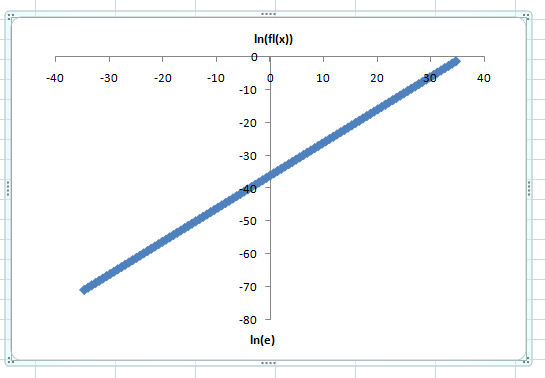
\includegraphics[width=\textwidth]{grafico}
\end{figure}

\item Indique la relación del gráfico anterior con la propiedad \\
$\mid fl(x)-x \mid \leq 0,5 \epsilon_{mach} \mid x \mid$
\end{enumerate}

\section{Parte II: Pérdida de Significancia}

\subsection{Pregunta 1}
\begin{enumerate}[a)]
\item Con la ayuda de Python o Matlab, evalúe la función en $x=10^{-t}$, donde $t \in \{1, 2, 3,...,20\}$ \\
Evaluando la función con la ayuda de Python (Código en Anexo) se presenta un extracto de la tabla de resultados para los distintos valores de $t$:
\begin{center}
\begin{tabular}{|c|c|c|}
\cline{1-3}
p & $x=10^{-t}$ & $y(x)$  \\
\cline{1-3}
1 & 0.10000000000000000000 & -0.49874791371143462 \\
\cline{1-3}
2 & 0.01000000000000000000 & -0.49998749979095553 \\
\cline{1-3}
3 & 0.00100000000000000000 & -0.49999987501428939 \\
\cline{1-3}
4 & 0.00010000000000000000 & -0.49999999362793118 \\
\cline{1-3}
5 & 0.00001000000000000000 & -0.50000004133685227 \\
\cline{1-3}
6 & 0.00000100000000000000 & -0.50004445029083722 \\
\cline{1-3}
7 & 0.00000010000000000000 & -0.51070259132756868 \\
\cline{1-3}
8 & 0.00000001000000000000 & 0.0 \\
\cline{1-3}
9 & 0.00000000100000000000 & 0.0 \\
\cline{1-3}
19 & 0.00000000000000000010 & 0.0 \\
\cline{1-3}
20 & 0.00000000000000000001 & 0.0 \\
\cline{1-3}
\end{tabular}
\end{center}

Se aprecia que a partir de $t=8$ existe una falta de precisión del computador, específicamente cuando se calcula la $sec(x)$ en la función, dando como resultado siempre $1.0$, es decir, cuando se calcula el numerador de la función ($1-sec(x)$) queda como resultado $0.0$.

\item Encuentre \textbf{dos} representaciones alternativas para eliminar los errores de cancelación del Factor Mavillano. \\
Primera representación:
$$y(x)= \left(\frac{cos(x)}{sen(x)}\right)^2 - \frac{cos(x)}{sen(x)^2}$$ \\
Segunda Representación:
$$y(x)=$$

\item Calcule los errores relativos entre el valor aritmético y sus representaciones alternativas para cada evaluación realizada. Concluya al respecto.

\item Analice como afecta $\epsilon_{mach}$ en lo realizado anteriormente ¿Cómo reacciona el error en cálculos de arrastre?

\end{enumerate}

\section{Conclusión}

\section{Referencias}
\begin{enumerate}
\item Timothy Sauer; Numerical Analysis, 2012, 2nd ed., p. 5-14
\end{enumerate}

\section{Anexo}
Para la resolución de los problemas de utilizaron los siguientes códigos de  \textit{Python}:

\begin{itemize}
\item Parte I, Pregunta 1, b)
\begin{verbatim}
# Item 1
print("i.1")
print("((1 + 2**(-52)) - 1) + 2**(-54) + 1")
r1 = 1 + 2**(-52)
print("((" + str(r1) + ") - 1) + 2**(-54) + 1")
r1 -= 1
print("(" + str(r1) + ") + 2**(-54) + 1")
r1 += 2**(-54)
print(str(r1) + " + 1")
r1 += 1
print(str(r1))
print("i.2")
print("((1 + 2**(-54)) - 1) + 2**(-52) + 1")
r1 = 1 + 2**(-54)
print("((" + str(r1) + ") - 1) + 2**(-52) + 1")
r1 -= 1
print("(" + str(r1) + ") + 2**(-52) + 1")
r1 += 2**(-52)
print(str(r1) + " + 1")
r1 += 1
print(str(r1))
print("")
# Item 2
print("ii.1")
print("(5 - 4) + 2**(-52)")
r1 = 5 - 4
print (str(r1) + " + 2**(-52)")
r1 += 2**(-52)
print(r1)
print("ii.2")
print("5 - (4 - 2**(-52))")
r1 = 4 - 2**(-52)
print("5 - " + str(r1))
r1 = 5 - r1
print(r1)
print("")
#Item 3
print("iii.1")
print("(2**(53) + (-2**(53)) + (1 + .5 + .25)")
r1 = 2**(53) + (-2**(53))
r2 = 1 + .5 + .25
print(str(r1) + " + " + str(r2))
print(str(r1 + r2))
print("iii.2")
print("(2**(53) + (1 + .5 + .25)) - 2**(53)")
r1 = 2**(53) + (1 + .5 + .25)
print(str(r1) + " - 2**(53)")
r1 = r1 - 2**(53)
print(r1)
\end{verbatim}
\item Parte I, Pregunta 2, b)
\begin{verbatim}
e_mach = 2**(-52)
x = 1.9999999999999
while(((x + e_mach) - x) != 0):
	x += e_mach
	print(x)
print("El menor numero en el cual la suma no es representables es: " + str(x))

\end{verbatim}
\item Parte I, Pregunta 2, c)
\begin{verbatim}
e_mach = 2**(-52)
x_1 = 0.9999999999999
x_2 = x_1
while(((x_2 + e_mach/2) - x_2) != 0):
	x_1 = x_2
	x_2 += e_mach/2
	print(x_2)
print("El mayor numero en el cual la suma es representables es: " + str(x_1))
\end{verbatim}
\item Parte I, Pregunta 3, a)
\begin{verbatim}
def epsilon(fl):
	if(fl >= 1):
		exp = 0
		while(fl >= 2 ** (exp + 1)):
			exp += 1
	else:
		exp = -1
		while(fl <= 2 **(exp - 1)):
			exp -= 1
	exp -= 52
	return 2**exp
\end{verbatim}
\item Parte I, Pregunta 3, b)
\begin{verbatim}
from parte1_pregunta3_a import epsilon

print("| i | e |")
for i in range (-50, 51):
	print("| " + str(i) + " | " + str(epsilon(2**(i))) + " |")
\end{verbatim}
\item Parte II, Pregunta 1, a)
\begin{verbatim}
from math import *
def Mavillan ():
    for i in range(1,21):
        a = 10**(-i)
        b = (1-(1/cos(a)))/((tan(a)**2))
        print(b)
    print ("\n")
Mavillan()
\end{verbatim}

\item Parte II, Pregunta 1, b)
\begin{verbatim}
from math import *
def Mavillan2():
    for i in range(1,21):
        a = 10**(-i)
        b = ((cos(a)/sin(a))**2)-(cos(a)/(sin(a))**2)
        print(b)
    print ("\n")
Mavillan2()
\end{verbatim}

\end{itemize}
\end{document}